\chapter{Luogo delle radici}


Eistono due tipologie di luoghi delle radici, diretto e indiretto.

Avendo un guadagno ad anello:
\begin{align}
  L(s) = G(s)H(s) = K_1 \frac{(s-z_1)\dots(s-z_m)}{(s-p_1)\dots(s-p_m)} = K_1G_1(s)
\end{align}

Il luogo delle radici diretto `e descritto da $1 + K_1G_1(s) = 0$ con $K_1$ che varia 
da $0$ a $+\infty$.

Il luogo delle radici inverse ha invece $1 + \frac{1}{K_1G_1(s)} = 0$ con $K_1$ che varia
da $0$ a $-\infty$.


\section{Propriet\`a del luogo delle radici}
\begin{itemize}
  \item Il luogo delle radici ha tanti rami quanti sono i poli di $G_1(s)$.
  \item Ogni ramo parte da un polo di $G_1(s)$ e tende ad un zero di $G_1(s)$.
  \item Il luogo delle radici \`e simmetrico rispetto all'asse reale.
  \item Nel luogo diretto, un punto dell'asse reale fa parte del luogo delle radici se alla sua destra ci sono un numero dispari di poli e zeri.
  \item Nel luogo inverso, un punto dell'asse reale fa parte del luogo delle radici se alla sua destra ci sono un numero pari di poli e zeri.
\end{itemize}




\subsection{Angoli luogo diretto}

\begin{align}
  \{ \text{Angoli partenza da $p_i$} \} = \varphi_i = \pi + \sum_{j = 1}^m \arg(p_i - z_j) - \sum_{j \neq 1} \arg(p_i - p_j) \\
  \{ \text{Angoli arrivo in $z_i$} \} = \psi_i = \pi + \sum_{j = 1}^m \arg(z_i - p_j) - \sum_{j \neq 1} \arg(z_i - z_j)
\end{align}



\subsection{Angoli luogo inverso}
Qui s imetto 0 al posto di $\pi$:

\begin{align}
  \{ \text{Angoli partenza da $p_i$} \} = \varphi_i = \sum_{j = 1}^m \arg(p_i - z_j) - \sum_{j \neq 1} \arg(p_i - p_j) \\
  \{ \text{Angoli arrivo in $z_i$} \} = \psi_i = \sum_{j = 1}^m \arg(z_i - p_j) - \sum_{j \neq 1} \arg(z_i - z_j)
\end{align}


\subsection{Molteplicit\`a}
Se il polo $p_i$ ha molteplicit\`a $h > 1$:
\begin{align}
  h \varphi_i = \pi + \sum_{j = 1}^m \arg(p_i - z_j) - \sum_{j \neq 1} \arg(p_i - p_j) \mod(2\pi) \\
  h \psi_i = \pi + \sum_{j = 1}^m \arg(z_i - p_j) - \sum_{j \neq 1} \arg(z_i - z_j) \mod(2\pi) 
\end{align}



\section{Asintoti del luogo delle radici}
Punto nell'asse reale dove si forma una stella di asintoti(di raggi):
\begin{align}
  \sigma_a = \frac{\sum_{i-1}^n p_i - \sum_{i=1}^M z_i}{n-m}
\end{align}

Gli angoli degli asintoti nel luogo delle radici diretto sono:
\begin{align}
  \vartheta_{a, v} = \frac{(2v+1)\pi}{n-m} \quad v = 0, 1, \dots, n-m-1
\end{align}

\begin{figure}[h!]
  \centering
  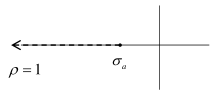
\includegraphics[width=0.15\linewidth]{images/luogo_delle_radici_grado_relativo_1.png}
  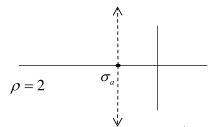
\includegraphics[width=0.15\linewidth]{images/luogo_delle_radici_grado_relativo_2.png}
  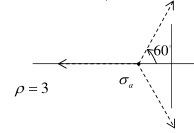
\includegraphics[width=0.15\linewidth]{images/luogo_delle_radici_grado_relativo_3.png}
  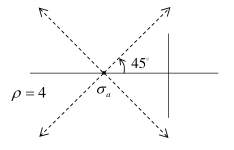
\includegraphics[width=0.15\linewidth]{images/luogo_delle_radici_grado_relativo_4.png}
  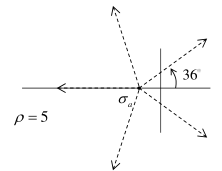
\includegraphics[width=0.15\linewidth]{images/luogo_delle_radici_grado_relativo_5.png}
\end{figure}

Se il luogo dovesse essere inverso:
\begin{align}
  \vartheta_{a, v} = \frac{2v\pi}{n-m} \quad v = 0, 1, \dots, n-m-1
\end{align}


\begin{figure}[h!]
  \centering
  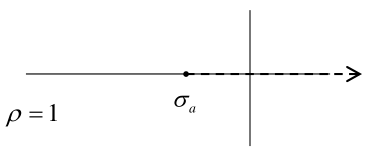
\includegraphics[width=0.15\linewidth]{images/luogo_delle_radici_grado_relativo_1_inverso.png}
  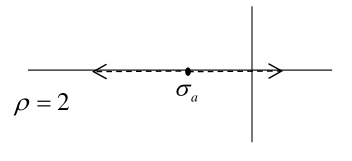
\includegraphics[width=0.15\linewidth]{images/luogo_delle_radici_grado_relativo_2_inverso.png}
  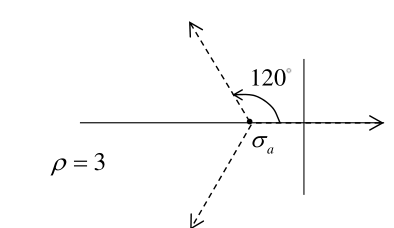
\includegraphics[width=0.15\linewidth]{images/luogo_delle_radici_grado_relativo_3_inverso.png}
  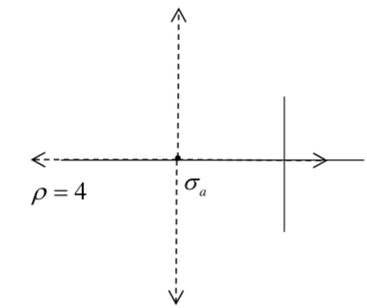
\includegraphics[width=0.15\linewidth]{images/luogo_delle_radici_grado_relativo_4_inverso.png}
  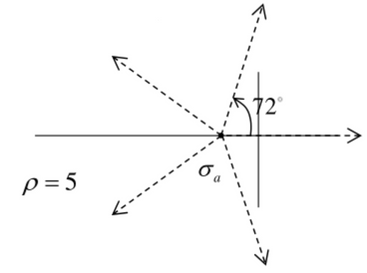
\includegraphics[width=0.15\linewidth]{images/luogo_delle_radici_grado_relativo_5_inverso.png}
\end{figure}




